%% BioMed_Central_Tex_Template_v1.06
%%                                      %
%  bmc_article.tex            ver: 1.06 %
%                                       %

%%IMPORTANT: do not delete the first line of this template
%%It must be present to enable the BMC Submission system to
%%recognise this template!!

%%%%%%%%%%%%%%%%%%%%%%%%%%%%%%%%%%%%%%%%%
%%                                     %%
%%  LaTeX template for BioMed Central  %%
%%     journal article submissions     %%
%%                                     %%
%%          <8 June 2012>              %%
%%                                     %%
%%                                     %%
%%%%%%%%%%%%%%%%%%%%%%%%%%%%%%%%%%%%%%%%%


%%%%%%%%%%%%%%%%%%%%%%%%%%%%%%%%%%%%%%%%%%%%%%%%%%%%%%%%%%%%%%%%%%%%%
%%                                                                 %%
%% For instructions on how to fill out this Tex template           %%
%% document please refer to Readme.html and the instructions for   %%
%% authors page on the biomed central website                      %%
%% http://www.biomedcentral.com/info/authors/                      %%
%%                                                                 %%
%% Please do not use \input{...} to include other tex files.       %%
%% Submit your LaTeX manuscript as one .tex document.              %%
%%                                                                 %%
%% All additional figures and files should be attached             %%
%% separately and not embedded in the \TeX\ document itself.       %%
%%                                                                 %%
%% BioMed Central currently use the MikTex distribution of         %%
%% TeX for Windows) of TeX and LaTeX.  This is available from      %%
%% http://www.miktex.org                                           %%
%%                                                                 %%
%%%%%%%%%%%%%%%%%%%%%%%%%%%%%%%%%%%%%%%%%%%%%%%%%%%%%%%%%%%%%%%%%%%%%

%%% additional documentclass options:
%  [doublespacing]
%  [linenumbers]   - put the line numbers on margins

%%% loading packages, author definitions

%\documentclass[twocolumn]{bmcart}% uncomment this for twocolumn layout and comment line below
\documentclass{bmcart}

%%% Load packages
%\usepackage{amsthm,amsmath}
%\RequirePackage{natbib}
%\RequirePackage{hyperref}
\usepackage[utf8]{inputenc} %unicode support
%\usepackage[applemac]{inputenc} %applemac support if unicode package fails
%\usepackage[latin1]{inputenc} %UNIX support if unicode package fails


%%%%%%%%%%%%%%%%%%%%%%%%%%%%%%%%%%%%%%%%%%%%%%%%%
%%                                             %%
%%  If you wish to display your graphics for   %%
%%  your own use using includegraphic or       %%
%%  includegraphics, then comment out the      %%
%%  following two lines of code.               %%
%%  NB: These line *must* be included when     %%
%%  submitting to BMC.                         %%
%%  All figure files must be submitted as      %%
%%  separate graphics through the BMC          %%
%%  submission process, not included in the    %%
%%  submitted article.                         %%
%%                                             %%
%%%%%%%%%%%%%%%%%%%%%%%%%%%%%%%%%%%%%%%%%%%%%%%%%


% \def\includegraphic{}
% \def\includegraphics{}



%%% Put your definitions there:
\startlocaldefs

\usepackage{xspace}
\newcommand{\disco}{{\it DiscoSnp}\xspace}
\newcommand{\discopp}{{\it DiscoSnp++}\xspace}
\newcommand{\co}{{\it cortex}\xspace}
\usepackage{xcolor}
\definecolor{my_green}{rgb}{0,0.5,0}
\usepackage{graphicx}
\usepackage{color}
\usepackage{url}
\endlocaldefs


%%% Begin ...
\begin{document}

%%% Start of article front matter
\begin{frontmatter}

\begin{fmbox}
\dochead{Technical Note}

%%%%%%%%%%%%%%%%%%%%%%%%%%%%%%%%%%%%%%%%%%%%%%
%%                                          %%
%% Enter the title of your article here     %%
%%                                          %%
%%%%%%%%%%%%%%%%%%%%%%%%%%%%%%%%%%%%%%%%%%%%%%

\title{{\it DiscoSnp++}: detection of all kind of SNPs and of indels from raw unassembled read set(s)}

%%%%%%%%%%%%%%%%%%%%%%%%%%%%%%%%%%%%%%%%%%%%%%
%%                                          %%
%% Enter the authors here                   %%
%%                                          %%
%% Specify information, if available,       %%
%% in the form:                             %%
%%   <key>={<id1>,<id2>}                    %%
%%   <key>=                                 %%
%% Comment or delete the keys which are     %%
%% not used. Repeat \author command as much %%
%% as required.                             %%
%%                                          %%
%%%%%%%%%%%%%%%%%%%%%%%%%%%%%%%%%%%%%%%%%%%%%%

\author[
   addressref={aff1},                   % id's of addresses, e.g. {aff1,aff2}
   corref={aff1},                       % id of corresponding address, if any
   % noteref={n1},                        % id's of article notes, if any
   email={pierre.peterlongo@inria.fr}   % email address
]{\inits{PP}\fnm{Pierre} \snm{Peterlongo}}
 \author[
    addressref={aff1},
    email={erwan.drezen@inria.fr}
 ]{\inits{ED}\fnm{Erwan} \snm{Drezen}}
 \author[
    addressref={aff1},
    email={claire.lemaitre@inria.fr}
 ]{\inits{ED}\fnm{Claire} \snm{Lemaitre}}
 \author[
    addressref={aff1},
    email={chloe.riou@inria.fr}
 ]{\inits{ED}\fnm{Chloé} \snm{Riou}}

%%%%%%%%%%%%%%%%%%%%%%%%%%%%%%%%%%%%%%%%%%%%%%
%%                                          %%
%% Enter the authors' addresses here        %%
%%                                          %%
%% Repeat \address commands as much as      %%
%% required.                                %%
%%                                          %%
%%%%%%%%%%%%%%%%%%%%%%%%%%%%%%%%%%%%%%%%%%%%%%

\address[id=aff1]{%                           % unique id
  \orgname{GenScale, INRIA Rennes Bretagne-Atlantique, IRISA}, % university, etc
  \street{Campus de Beaulieu},                     %
  %\postcode{}                                % post or zip code
  \city{Rennes},                              % city
  \cny{France}                                    % country
}
% \address[id=aff2]{%
%   \orgname{Marine Ecology Department, Institute of Marine Sciences Kiel},
%   \street{D\"{u}sternbrooker Weg 20},
%   \postcode{24105}
%   \city{Kiel},
%   \cny{Germany}
% }

%%%%%%%%%%%%%%%%%%%%%%%%%%%%%%%%%%%%%%%%%%%%%%
%%                                          %%
%% Enter short notes here                   %%
%%                                          %%
%% Short notes will be after addresses      %%
%% on first page.                           %%
%%                                          %%
%%%%%%%%%%%%%%%%%%%%%%%%%%%%%%%%%%%%%%%%%%%%%%

\begin{artnotes}
%\note{Sample of title note}     % note to the article
% \note[id=n1]{Equal contributor} % note, connected to author
\end{artnotes}

\end{fmbox}% comment this for two column layout

%%%%%%%%%%%%%%%%%%%%%%%%%%%%%%%%%%%%%%%%%%%%%%
%%                                          %%
%% The Abstract begins here                 %%
%%                                          %%
%% Please refer to the Instructions for     %%
%% authors on http://www.biomedcentral.com  %%
%% and include the section headings         %%
%% accordingly for your article type.       %%
%%                                          %%
%%%%%%%%%%%%%%%%%%%%%%%%%%%%%%%%%%%%%%%%%%%%%%

\begin{abstractbox}

\begin{abstract} % abstract

NGS data provides an unprecedented access to life mechanisms. In particular these data enable to detect polymorphisms such as SNPs and indels. 
As these polymorphisms represent a fundamental source of information in agronomy, environment or medicine,  their detection is a routine task with NGS data. The main methods for their prediction usually need a reference genome. However, non-model organisms and highly divergent genomes such as in cancer studies are more and more investigated. 
\disco tool had been successfully applied to predicts isolated SNPs from raw read set(s) (1 to $n$) without the need of a reference genome. 
We propose \discopp, the successor of \disco, which has the advantage of a new algorithm design that reduces time and memory consumption, detects all kind of SNP, detects indels, genotypes results and output a VCF file. Results show that \discopp performs better than state-of-the-art methods both in term of results quality and computational resources. 

\end{abstract}

%%%%%%%%%%%%%%%%%%%%%%%%%%%%%%%%%%%%%%%%%%%%%%
%%                                          %%
%% The keywords begin here                  %%
%%                                          %%
%% Put each keyword in separate \kwd{}.     %%
%%                                          %%
%%%%%%%%%%%%%%%%%%%%%%%%%%%%%%%%%%%%%%%%%%%%%%

\begin{keyword}
\kwd{SNP}
\kwd{Indel}
\kwd{reference-free}
\end{keyword}

% MSC classifications codes, if any
%\begin{keyword}[class=AMS]
%\kwd[Primary ]{}
%\kwd{}
%\kwd[; secondary ]{}
%\end{keyword}

\end{abstractbox}
%
%\end{fmbox}% uncomment this for twcolumn layout

\end{frontmatter}

%%%%%%%%%%%%%%%%%%%%%%%%%%%%%%%%%%%%%%%%%%%%%%
%%                                          %%
%% The Main Body begins here                %%
%%                                          %%
%% Please refer to the instructions for     %%
%% authors on:                              %%
%% http://www.biomedcentral.com/info/authors%%
%% and include the section headings         %%
%% accordingly for your article type.       %%
%%                                          %%
%% See the Results and Discussion section   %%
%% for details on how to create sub-sections%%
%%                                          %%
%% use \cite{...} to cite references        %%
%%  \cite{koon} and                         %%
%%  \cite{oreg,khar,zvai,xjon,schn,pond}    %%
%%  \nocite{smith,marg,hunn,advi,koha,mouse}%%
%%                                          %%
%%%%%%%%%%%%%%%%%%%%%%%%%%%%%%%%%%%%%%%%%%%%%%

%%%%%%%%%%%%%%%%%%%%%%%%% start of article main body
% <put your article body there>

%%%%%%%%%%%%%%%%
%% Background %%
%%

\section*{Introduction}

NGS data provides an unprecedented access to life mechanisms. In particular these data enable to asses genetic differences between chromosomes, individuals or species. 
Such polymorphisms represent a fundamental source of information in many aspect of biology with numerous applications in agronomy, environment or medicine. 

Within the democratization of the sequencing provided by the NGS technologies, determining genetic differences as SNPs or indels has become a routine task the last decade. There exists large number of applications designed for predicting such polymorphisms. Mostly, these methods are based on the use of a reference genome as this is a case for GATK~\cite{gatk} or SamTools~\cite{Li2009} mapping sequenced reads or by mapping partial assemblies as for DISCOVAR~\cite{Weisenfeld2014} or FERMI~\cite{Li2012} to cite a few. Basically they first map the NGS reads on the reference and in a second phase the differences between the reference and the reads are analyzed to be classified and ranked with respect to distinct criteria, and output. 

These methods are highly accepted and used. However, they present severe drawbacks. First they suffer from the mapping quality. Highly repeated regions of the reference genome are difficult to map with a high degree of confidence.  Polymorphism detected from these repeated regions may be erroneous as the quantification of mapped reads is erroneous and as the differences between occurrences of the repeats can be interpreted as the output polymorphism. Secondly, they suffer from the fact that they need a high quality reference genome. This evident and strong condition limit the application to reference species. 

In practice, biologists are more and more working on species for which there exists no confident reference genome. Additionally, despite large improvements in the sequencing techniques this last decade, reconstructing a perfect and complete genome from reads remains a highly complex task~\cite{assemblathon2}. In this context there is an important need for \emph{reference-free} methods detecting SNPs and indels, directly from NGS reads, without requiring an assembled reference sequence. A method may consists in first assemble reads before to map them back on the so obtained reference, as this is the case in~\cite{Willing2011}. However such methods cumulate both the assembly and the mapping difficulties. In this manuscript, we refer to such methods as the \emph{hybrid} strategy. 

A few methods~\cite{Peterlongo2010,iqbal2012novo,Leggett2013,Nordstrom2013,Kissplice} were proposed for \emph{de-novo} detection of polymorphism.  All these methods are based on the use of the \emph{de Bruijn graph}, i.e. a directed graph where the set of vertices corresponds to the set of words of length $k$ ($k$-mers) contained in the reads, and there is an edge between two $k$-mers if they overlap on $k-1$ nucleotides. In this data structure polymorphism generate recognizable patterns called the \emph{bubbles}. These tools detects and analyze such bubbles in order to decide their origin (sequencing errors, polymorphism from inexact repeats, real SNP or indel). 

We recently proposed \disco, a \emph{reference-free} method for detecting isolated SNPs~\cite{Uricaru2014a}. The \disco approach outperforms other \emph{reference-free} methods both in term of computational needs and in term of results quality. Its main features are \textbf{1}/ its extremely low memory usage (several billion reads may be analyzed with no more than 6 GB RAM memory), \textbf{2}/ its high execution speed, \textbf{3}/ its high precision and recall, \textbf{4}/ the precision of the score assigned to each predicted SNP, \textbf{5}/ the fact that is can be applied on one to $n$ read sets, and \textbf{6}/ the kind of SNPs it detects, called \emph{isolated}. Isolated SNPs are SNPs that are distant to the left and to the right by at least $k$ nucleotides from any other polymorphism, with $k$ one of the main parameters of a SNP detection tool. Isolated SNPs have the advantage to be easily amplified by PCR. However isolated SNPs do jot represent all SNPs. In particular in case of highly polymorphic genomes and in case of numerous distinct genomes, only a fraction of SNPs are isolated and so detected by \disco.


In this paper, we present \discopp that is an extension of the \disco tool. The tool was re-implemented from scratch using the GATB library~\cite{Drezen2014}. Except the running time that has been even improved, the detection of isolated SNPs remains exactly the same with \disco and \discopp. Additionally, \discopp detects new kind of variants and it may proposes a VCF of the predicted variants.  


The \disco tool is based on the analysis of the de Bruijn Graph (dBG) for predicting \emph{isolated SNPs}. An \emph{isolated SNP} is a SNPs that is at least $k$ nucleotides apart from any other polymorphism, with $k$ the size of the $k$-mers used in the dBG. 

In a dBG, a \emph{bubble} denotes a path in the graph which diverges into two distinct paths before to merge back. In the dBG of one or several read sets, a specific motif witnesses the presence of isolated SNPs. This motif is a bubble whose the two distinct paths are composed of exactly $k$ nodes. Figure~\ref{fig:basical_bubble}.a shows a toy example of such a bubble. 



\disco works as follows: \textbf{(1)} build the dBG of the input dataset(s);  \textbf{(2)} detect motifs witnessing the presence of isolated SNPs; \textbf{(3)} output their corresponding sequences together with the contig they belong to; \textbf{(4)} map back the reads of all read sets on the sequences of these motifs, mainly in order to recover the coverage and read quality per read sets. 

The final output is a Fasta file containing for each predicted SNP a couple of sequence distinct by a unique polymorphic nucleotide. Among other informations, the headers of the sequences provides the coverage per allele and per read set. 

A score between 0 and 1 is affected to each SNP. This score is the Phi coefficient of the table of read counts, computed as follows: $\sqrt{\frac{\chi^2}{n}}$. When two or more read sets are used, this score enables to distinguish predicted SNPs due to inexact repeats from real SNPs as inexact repeats are likely to have a similar profile in each dataset.  



\section*{Improvements in \discopp}
Several improvements are proposed in \discopp. In particular the type of predicted variant is not limited to isolated SNPs. In addition, a VCF file is output, providing among others the genotype of the predictions.

\subsection*{Detecting close SNPs and indels}


Conversely to isolated SNPs, \emph{close} SNPs are SNPs close to each other or to any source of polymorphism by less than $k$ nucleotides.
In the dBG, close SNPs generate a bubble whose the two distinct paths are composed of more than $k$ nodes. Figure~\ref{fig:basical_bubble}.b shows a toy example of such a bubble.  
In \discopp, we extended the initial model detection in order to detect close SNPs in addition to isolated ones. The user may limit the maximal number of close SNPs that can be detected in a bubble. %This highly limit the computation time as well as the false positive rate. 

As presented Figure~\ref{fig:basical_bubble}.c, indels in data also generate bubbles in the dBG. The two paths of such bubbles are of distinct lengths. The smaller one is of size at most $k-1$ nodes. \discopp detects isolated indels in the dBG. The user limits the maximal size of the insertion. 

\subsection*{Predicting genotypes}
For each prediction, a genotype is provided (see Additional File 1 for details about the genotyping process). Users may deactivate genotyping, for instance when results are not predicted from diploid species.

\subsection*{Providing a VCF file}
The original \disco output is a fasta file. It contains a couple of sequences for each predicted variant. Headers of these sequences contain the read coverage and average read quality per variant and per input read set. The read coverage enables to provides a trustful ranking (see for instance the results presented Figure~\ref{fig:roc_human}).

In \discopp, in addition to the original fasta format, a VCF file is output. This file provides all pieces of information contained in the original fasta headers plus the genotyping values.


For creating the VCF file, a reference genome may be provided. In this case, for the variants successfully mapped on the reference, the VCF contains their genomic positions, the reference and the alternative allele unless none of the mapped sequences correspond to the reference genome, and additional mapping information (see Additional File 1 for details about the mapping process and details about the VCF content). 
If no reference is provided, this fields are replaced by dummy value '.'.




\section*{Results}
We propose results both on synthetic and on real datasets. Synthetic datasets offer a way to exactly compute the precision and the recall of \discopp and the state-of-the-art methods. Real datasets enable to assess the 

\subsection*{Results on synthetic datasets}
We first propose a bench of results based on synthetic datasets. As presented in the Additional File 1, these datasets are derived from real genomes, either from Escherichia Coli or or from the human chromosome 1. 

In these experiments, we generated the set of SNPs and indels. Thus we dispose from the exact and exhaustive list of variant to be found, and we are able to compute the precision and the recall of the predictions (see Additional File 1 for precision and recall computation details). We tested \discopp and \co and an hybrid method composed of SOAPdenovo2~\cite{luo2012soapdenovo2} for generating the assembly, Bowtie~\cite{langmead2012fast} for mapping the reads on the assembly, and GATK~\cite{gatk} for calling variants from this mapping. Presented results were obtained using the GATK \emph{UnifiedGenotyper} option. As presented in the Additional File 1, while following the GATK guidelines (including read realignment and using the \emph{HaplotypeCaller} option), the result quality is similar while the execution time is 3 times longer (from approximately 19h to 54h for the human chromosome 1 experiment). 

\subsubsection*{Two and more bacterial read sets}
We performed an experiment on a variable number of read sets. Each read set corresponds to a simulation of the sequencing of an Escherichia Coli individual. As presented in the Additional File 1, we simulated SNPs and indels such that the distribution inside a subset of individuals is realistic. 

Precision and recall results, presented Figure~\ref{fig:ncoli}, allow to draw conclusions while calling SNPs from several haploid individuals. On these data, both for calling SNPs or indels, the \co precision is perfect or nearly perfect, while recall highly decreases while the number of read sets increases, and it reaches less than 9\% for 30 genomes. 

For SNP calling, the hybrid strategy provides better results than \discopp: its recall is slightly better, and its precision remains more or less constant while the \discopp precision linearly decreases with the number of read sets. 


For indel calling, the hybrid strategy shows bad performances, that may be explained by the hardness of mapping read with indels. Conversely, \discopp presents high quality results both in term of precision and in term of recall. 


In short and in term of results quality only, for calling all SNPs from a large number of read sets from rather simple haploid genome, it is preferable to use an hybrid approach. However, we recall that for calling isolated SNPs only, \disco and the hybrid strategy lead to similar results (see~\cite{Uricaru2014a}). Note that the \disco results may be mimicked with \discopp by forbidding indels and close SNPs predictions. For indel calls, \discopp performs better than the other methods.

As shown Figure~\ref{fig:ncoliperf}, \discopp runs much faster that other methods and uses much less RAM memory. Moreover, one may also insist on the fact that \discopp is extremely simple to use. Table~\ref{tab:2colicmpxt}, showing the number of operations to perform for each method, witness this simplicity.

\subsubsection*{Two human datasets}
\label{ssec:twohumans}
For testing \discopp on a diploid genome, we propose an experiment based on the human chromosome 1, assembly GRCh37. Using SNPs predicted from the 1000 genome project, we simulated two individuals, generating 25,928 indels and 288,069 SNPs. The data simulation protocol is presented in the Additional File 1. 

Results while considering all predictions are presented Table~\ref{tab:humanresults}. 
The main conclusion is that, except for the hybrid approach that predicts few indels (40.97\%) with a high precision (96.15\%), other results do not show  notable difference, even if one may notice that precision is globally higher for indels, while the recall is higher for SNPs. 

Results presented Figure~\ref{fig:roc_human} provide additional pieces of information for the hybrid and the \discopp approaches. They show precision/recall values with respect to the ranking of the predictions (\co results are not ranked in this framework). Results show that the hybrid approach predictions are badly ranked: it appears that predictions showing the best scores are mainly false positives. Additionally, results show that the \discopp ranking is extremely efficient for separating false positives from true positives. Most of the predictions ranked with a score $>0.2$ are true positives (97.78\%  of the SNPs and 98.97\% of the indels). 

From these experiment on a complex eukaryotic species, one may conclude that \discopp overall results quality are more or less similar to results from other methods. However, it is the only tool with a reliable ranking of the results, enabling to select more than 50\% of the predictions with a nearly perfect precision.

As shown Figure~\ref{fig:perf_human}, \discopp runs much faster that other methods (respectively 3.6x and 17.5x times faster than \co and the hybrid approach) and uses much less RAM memory (respectively 36.2x and 22.9x times less memory than \co and the hybrid approach). 



TODO: genotyping resutls

\subsection*{Results on real datasets}
We used a set of biologically validated SNPs predicted from an artificial evolution study on Saccharomyces cerevisiae~\cite{Kvitek2013}. 
In this study, three glucose-limited, chemostat-evolved populations of haploid S288c, named
E1, E2 and E3, were sequenced every $\approx70$ generations, giving eight samples per population. Using a reference-based mapping approach, 110 mutations were discovered, among which only 33 have a minor allele frequency (MAF) $>10\%$ and 32 were confirmed by Sanger sequencing.  \discopp was run independently on populations E1, E2 and E3. For each population, \discopp was applied on the eight read sets corresponding to the eight time points, with the default parameters and c = 11. 

This dataset enables to evaluate \discopp SNP recall on real read datasets. Among 32 validated SNPs, 29 were predicted by \discopp, leading to an estimated recall of 90.7\%. Using parameter -b 2 leads to the detection of the unpredicted SNPs. The fact that these SNP are not detected with default (-b 1) parameter means that its bubble is symmetrically branching (see~\cite{Uricaru2014a} for an explanation of the branching filtration strategies). This reveals that these SNP are located in a complex region of the genome. 

Note that in the~\cite{Kvitek2013} study, no SNP with a MAF $<10\%$ were validated and no indel were validated, so we could not assess the precision of the \discopp predictions on this dataset.


\section*{Conclusion}
TODO
\section*{Availability and requirements}
\begin{itemize}
	\item \textbf{Project name:} \discopp
	\item \textbf{Operating systems}: Linux and osx;
	\item \textbf{Programming language}: C++ (main algorithms), bash and python;
	\item \textbf{Other requirement}: BWA~\cite{bwa} if users requires to map predictions on a reference genome while generating a VCF ouput;
	\item \textbf{License}: GNU AFFERO GENERAL PUBLIC LICENSE \url{gnu.org/licenses/agpl.html}
	\item \textbf{Any restrictions to use by non-academics}: license needed
\end{itemize}


\section*{Availability of supporting data}
[TODO if suitable for review]

The data sets supporting the results of this article are available in the [repository name] repository, [unique persistent identifier and hyperlink to dataset(s) in http:// format].


\section*{Abbreviations}
NGS: Next Generation Sequencing; SNP: Single Nucleotide Polymorphism; indel: insertion or deletion; PCR: Polymerase Chain Reaction; dBG: de Bruijn Graph; VCF: Variant Call Format; SAM: Sequence Alignment/Map; BAM: Binary Alignment/Map



% section section_name (end)



%%%%%%%%%%%%%%%%%%%%%%%%%%%%%%%%%%%%%%%%%%%%%%
%%                                          %%
%% Backmatter begins here                   %%
%%                                          %%
%%%%%%%%%%%%%%%%%%%%%%%%%%%%%%%%%%%%%%%%%%%%%%

\begin{backmatter}

\section*{Competing interests}
  The authors declare that they have no competing interests.

\section*{Author's contributions}
ED implemented the GATB library and re-coded \disco using this library, including parallelization and optimizations. PP designed and implemented the close SNPs and deletion detection algorithms. CL designed and implemented the genotyping algorithms. CR designed and implemented the VCF generation algorithms.  PP conceived and coordinated of the study, he wrote the manuscript draft. All authors participated in the writing, read and approved the final manuscript. 

\section*{Acknowledgements}
 We thank the \emph{GenOuest} (\url{genouest.org}) cluster team, who allowed us to perform all the tests. This work was supported by the French ANR-12-BS02-0008 \emph{Colib'read} project and by the ANR-12-EMMA-0019-01 \textbf{GATB} project.
 
%%%%%%%%%%%%%%%%%%%%%%%%%%%%%%%%%%%%%%%%%%%%%%%%%%%%%%%%%%%%%
%%                  The Bibliography                       %%
%%                                                         %%
%%  Bmc_mathpys.bst  will be used to                       %%
%%  create a .BBL file for submission.                     %%
%%  After submission of the .TEX file,                     %%
%%  you will be prompted to submit your .BBL file.         %%
%%                                                         %%
%%                                                         %%
%%  Note that the displayed Bibliography will not          %%
%%  necessarily be rendered by Latex exactly as specified  %%
%%  in the online Instructions for Authors.                %%
%%                                                         %%
%%%%%%%%%%%%%%%%%%%%%%%%%%%%%%%%%%%%%%%%%%%%%%%%%%%%%%%%%%%%%

% if your bibliography is in bibtex format, use those commands:
\bibliographystyle{bmc-mathphys} % Style BST file
\bibliography{discoSnppp_giga_science}      % Bibliography file (usually '*.bib' )

% or include bibliography directly:
% \begin{thebibliography}
% \bibitem{b1}
% \end{thebibliography}

%%%%%%%%%%%%%%%%%%%%%%%%%%%%%%%%%%%
%%                               %%
%% Figures                       %%
%%                               %%
%% NB: this is for captions and  %%
%% Titles. All graphics must be  %%
%% submitted separately and NOT  %%
%% included in the Tex document  %%
%%                               %%
%%%%%%%%%%%%%%%%%%%%%%%%%%%%%%%%%%%

%%
%% Do not use \listoffigures as most will included as separate files

\section*{Figures}

\begin{figure}[h!]  
\begin{minipage}[c]{0.05\textwidth}
\textbf{(a)}
\end{minipage}
\begin{minipage}[c]{0.90\textwidth}
\includegraphics[height=1.5cm]{figures/bubble_snp.png}
\end{minipage}\\

\begin{minipage}[c]{0.05\textwidth}
\textbf{(b)}
\end{minipage}
\begin{minipage}[c]{0.9\textwidth}

\includegraphics[height=1.5cm]{figures/bubble_close_snp.png}
\end{minipage}\\


\begin{minipage}[c]{0.05\textwidth}
\textbf{(c)}
\end{minipage}
\begin{minipage}[c]{0.9\textwidth}
\includegraphics[height=1.5cm]{figures/bubble_indel.png}
\end{minipage}\\

	
\caption{\csentence{Examples of dBG ($k=4$) bubbles due to SNP, close SNPs and indel.} \textbf{(a)} Bubble generated by an isolated SNP. Detected both by \disco and  \discopp. Prediction would be ACTG\textcolor{red}{A}CCTG and ACTG\textcolor{red}{T}CCTG. \textbf{(b)} Bubble generated by two close SNPs. Detected only by \discopp. Prediction would be ACTG\textcolor{red}{A}C\textcolor{red}{C}TAAT and ACTG\textcolor{red}{T}C\textcolor{red}{G}TAAT. \textbf{(c)} Bubble generated by an insertion. Detected only by \discopp. Prediction would be \textcolor{red}{ACTG}\textcolor{my_green}{ACCT} and \textcolor{red}{ACTG}TT\textcolor{my_green}{ACCT}. }
\label{fig:basical_bubble}
\end{figure}

\begin{figure}[h!]  
	\includegraphics[width=\linewidth]{../tests_n_coli_NAR/n_coli.png}
\caption{\csentence{\discopp, \co and hybrid strategy (SOAPdenovo2+GATK) results, depending on the number of input haploid individuals.} SOAPdenovo2 and GATK were launched with default parameters. For \discopp and \co, $k$-mers having three or fewer occurrences in all datasets were removed. Precision and recall: filled symbols represent the precision and empty symbols represent the recall. \textbf{Left:} results on SNPs predictions. \textbf{Right:} results on indels predictions. \label{fig:ncoli}}
\end{figure}


\begin{figure}[h!]  
	\includegraphics[width=\linewidth]{../tests_n_coli_NAR/perf_bact_article.png}
\caption{\csentence{Comparative memory and time performances, depending on the number of input haploid individuals.}\label{fig:ncoliperf}}
\end{figure}

\begin{figure}[h!]  
	\includegraphics[width=\linewidth]{../tests_human/results/roc_human.png}
\caption{\csentence{Comparative results of \discopp, \co,  and the hybrid SOAPdenovo2 + Bowtie2 + GATK approaches on the two diploid human chromosome 1 dataset.} Precision versus recall curves are obtained by ranking the predicted SNPs and indels. Each data point is obtained at a given rank threshold, where precision and recall values are computed for all SNPs with better ranks than this threshold. The dashed tail of the two \discopp curves denotes the predictions ranked with a threshold bellow $0.2$.
In this framework \co does not rank its predictions, its results are thus represented by a single point. \label{fig:roc_human}}
\end{figure}

\begin{figure}[h!]  
	\includegraphics[width=\linewidth]{../tests_human/results/perf_human_article.png}
\caption{\csentence{Comparative memory and time performances for comparing the two human datasets}\label{fig:perf_human}}
\end{figure}


%
% \begin{figure}[h!]
% \includegraphics[width=\linewidth]{../tests_n_coli_NAR/expes/res_b0_D_10_P_4_c_4_d_1.png}
% \caption{\csentence{AFAC Precision Recall of \discopp on a various number of E. Coli read sets.}
%       $b=0, D=10, P=4, c=4, d=1$.}
% \end{figure}
%
%
%
% \begin{figure}[h!]
% \includegraphics[width=\linewidth]{../tests_n_coli_NAR/expes/res_b1_D_10_P_4_c_4_d_1.png}
% \caption{\csentence{AFAC Precision Recall of \discopp on a various number of E. Coli read sets.}
%       $b=1, D=10, P=4, c=4, d=1$.}
% \end{figure}
%
%
% \begin{figure}[h!]
% \includegraphics[width=\linewidth]{../tests_n_coli_NAR/expes/res_b1_D_10_P_1_c_4_d_1.png}
% \caption{\csentence{AFAC Precision Recall of \discopp on a various number of E. Coli read sets.}
%       $b=1, D=10, P=1, c=4, d=1$.}
% \end{figure}
%
% \begin{figure}[h!]
% \includegraphics[width=\linewidth]{../tests_n_coli_NAR/expes/res_b2_D_10_P_4_c_4_d_1.png}
% \caption{\csentence{AFAC Precision Recall of \discopp on a various number of E. Coli read sets.}
%       $b=2, D=10, P=4, c=4, d=1$.}
% \end{figure}
%
%
% \begin{figure}[h!]
% \includegraphics[width=\linewidth]{../tests_n_coli_NAR/res_cortex_sabre/results.png}
% \caption{\csentence{AFAC Precision Recall of Cortex on a various number of E. Coli read sets.}
%       $k=31$.}
% \end{figure}


%%%%%%%%%%%%%%%%%%%%%%%%%%%%%%%%%%%
%%                               %%
%% Tables                        %%
%%                               %%
%%%%%%%%%%%%%%%%%%%%%%%%%%%%%%%%%%%

%% Use of \listoftables is discouraged.
%%
\section*{Tables}
\begin{table}[h!]
	\caption{XXX TODO RECOMPUTE THIS. Command line complexity in term of required number of command (including file formatting when necessary) while calling variants from 2 and 30 haploid genomes. See Additional File 1 for details.\label{tab:2colicmpxt}}
	\begin{tabular}{r|c|c}
		 & \begin{tabular}{c}Number of commands\\for two genomes\end{tabular} & \begin{tabular}{c}Number of commands\\for 30 genomes\end{tabular}\\\hline
		 Hybrid & 15  & 39\\
		 \co & 7 (+2 compilations) & 36 (+30 compilations) \\
		 \discopp & 2 & 2
	\end{tabular}
	\end{table}
	
	

\begin{table}[h!]
	\caption{Human chromosome 1 results.  \label{tab:humanresults} }
	\begin{tabular}{r|cc|cc}
		 & \multicolumn{2}{c|}{SNP} & \multicolumn{2}{c}{indels}\\
		 & Precision (\%) & Recall (\%) & Precision (\%) & Recall (\%) \\\hline
		 Hybrid & 71.60 & 78.59 & \textbf{96.15} & 40.97\\
		 \co& {73.19} & 67.34 & 86.65 & 63.25 \\
		 \discopp& 71.71 & \textbf{78.88} & 75.86 & \textbf{71.15} \\\hline
		 \discopp (rank $>$ 2)& 97.78 & 64.39 & 98.97 & 57.78 
	\end{tabular}
	\end{table}
% \begin{table}[h!]
% \caption{Sample table title. This is where the description of the table should go.}
%       \begin{tabular}{cccc}
%         \hline
%            & B1  &B2   & B3\\ \hline
%         A1 & 0.1 & 0.2 & 0.3\\
%         A2 & ... & ..  & .\\
%         A3 & ..  & .   & .\\ \hline
%       \end{tabular}
% \end{table}

%%%%%%%%%%%%%%%%%%%%%%%%%%%%%%%%%%%
%%                               %%
%% Additional Files              %%
%%                               %%
%%%%%%%%%%%%%%%%%%%%%%%%%%%%%%%%%%%

\section*{Additional Files}
  \subsection*{Additional file 1 --- Sample additional file title}
    Additional file descriptions text (including details of how to
    view the file, if it is in a non-standard format or the file extension).  This might
    refer to a multi-page table or a figure.
  %
  % \subsection*{Additional file 2 --- Sample additional file title}
  %   Additional file descriptions text.


\end{backmatter}
\end{document}
